% !TEX root = mythesis.tex

%==============================================================================
\chapter{Introduction}
\label{sec:intro}
%==============================================================================
\begin{figure}[h!]
\centering
  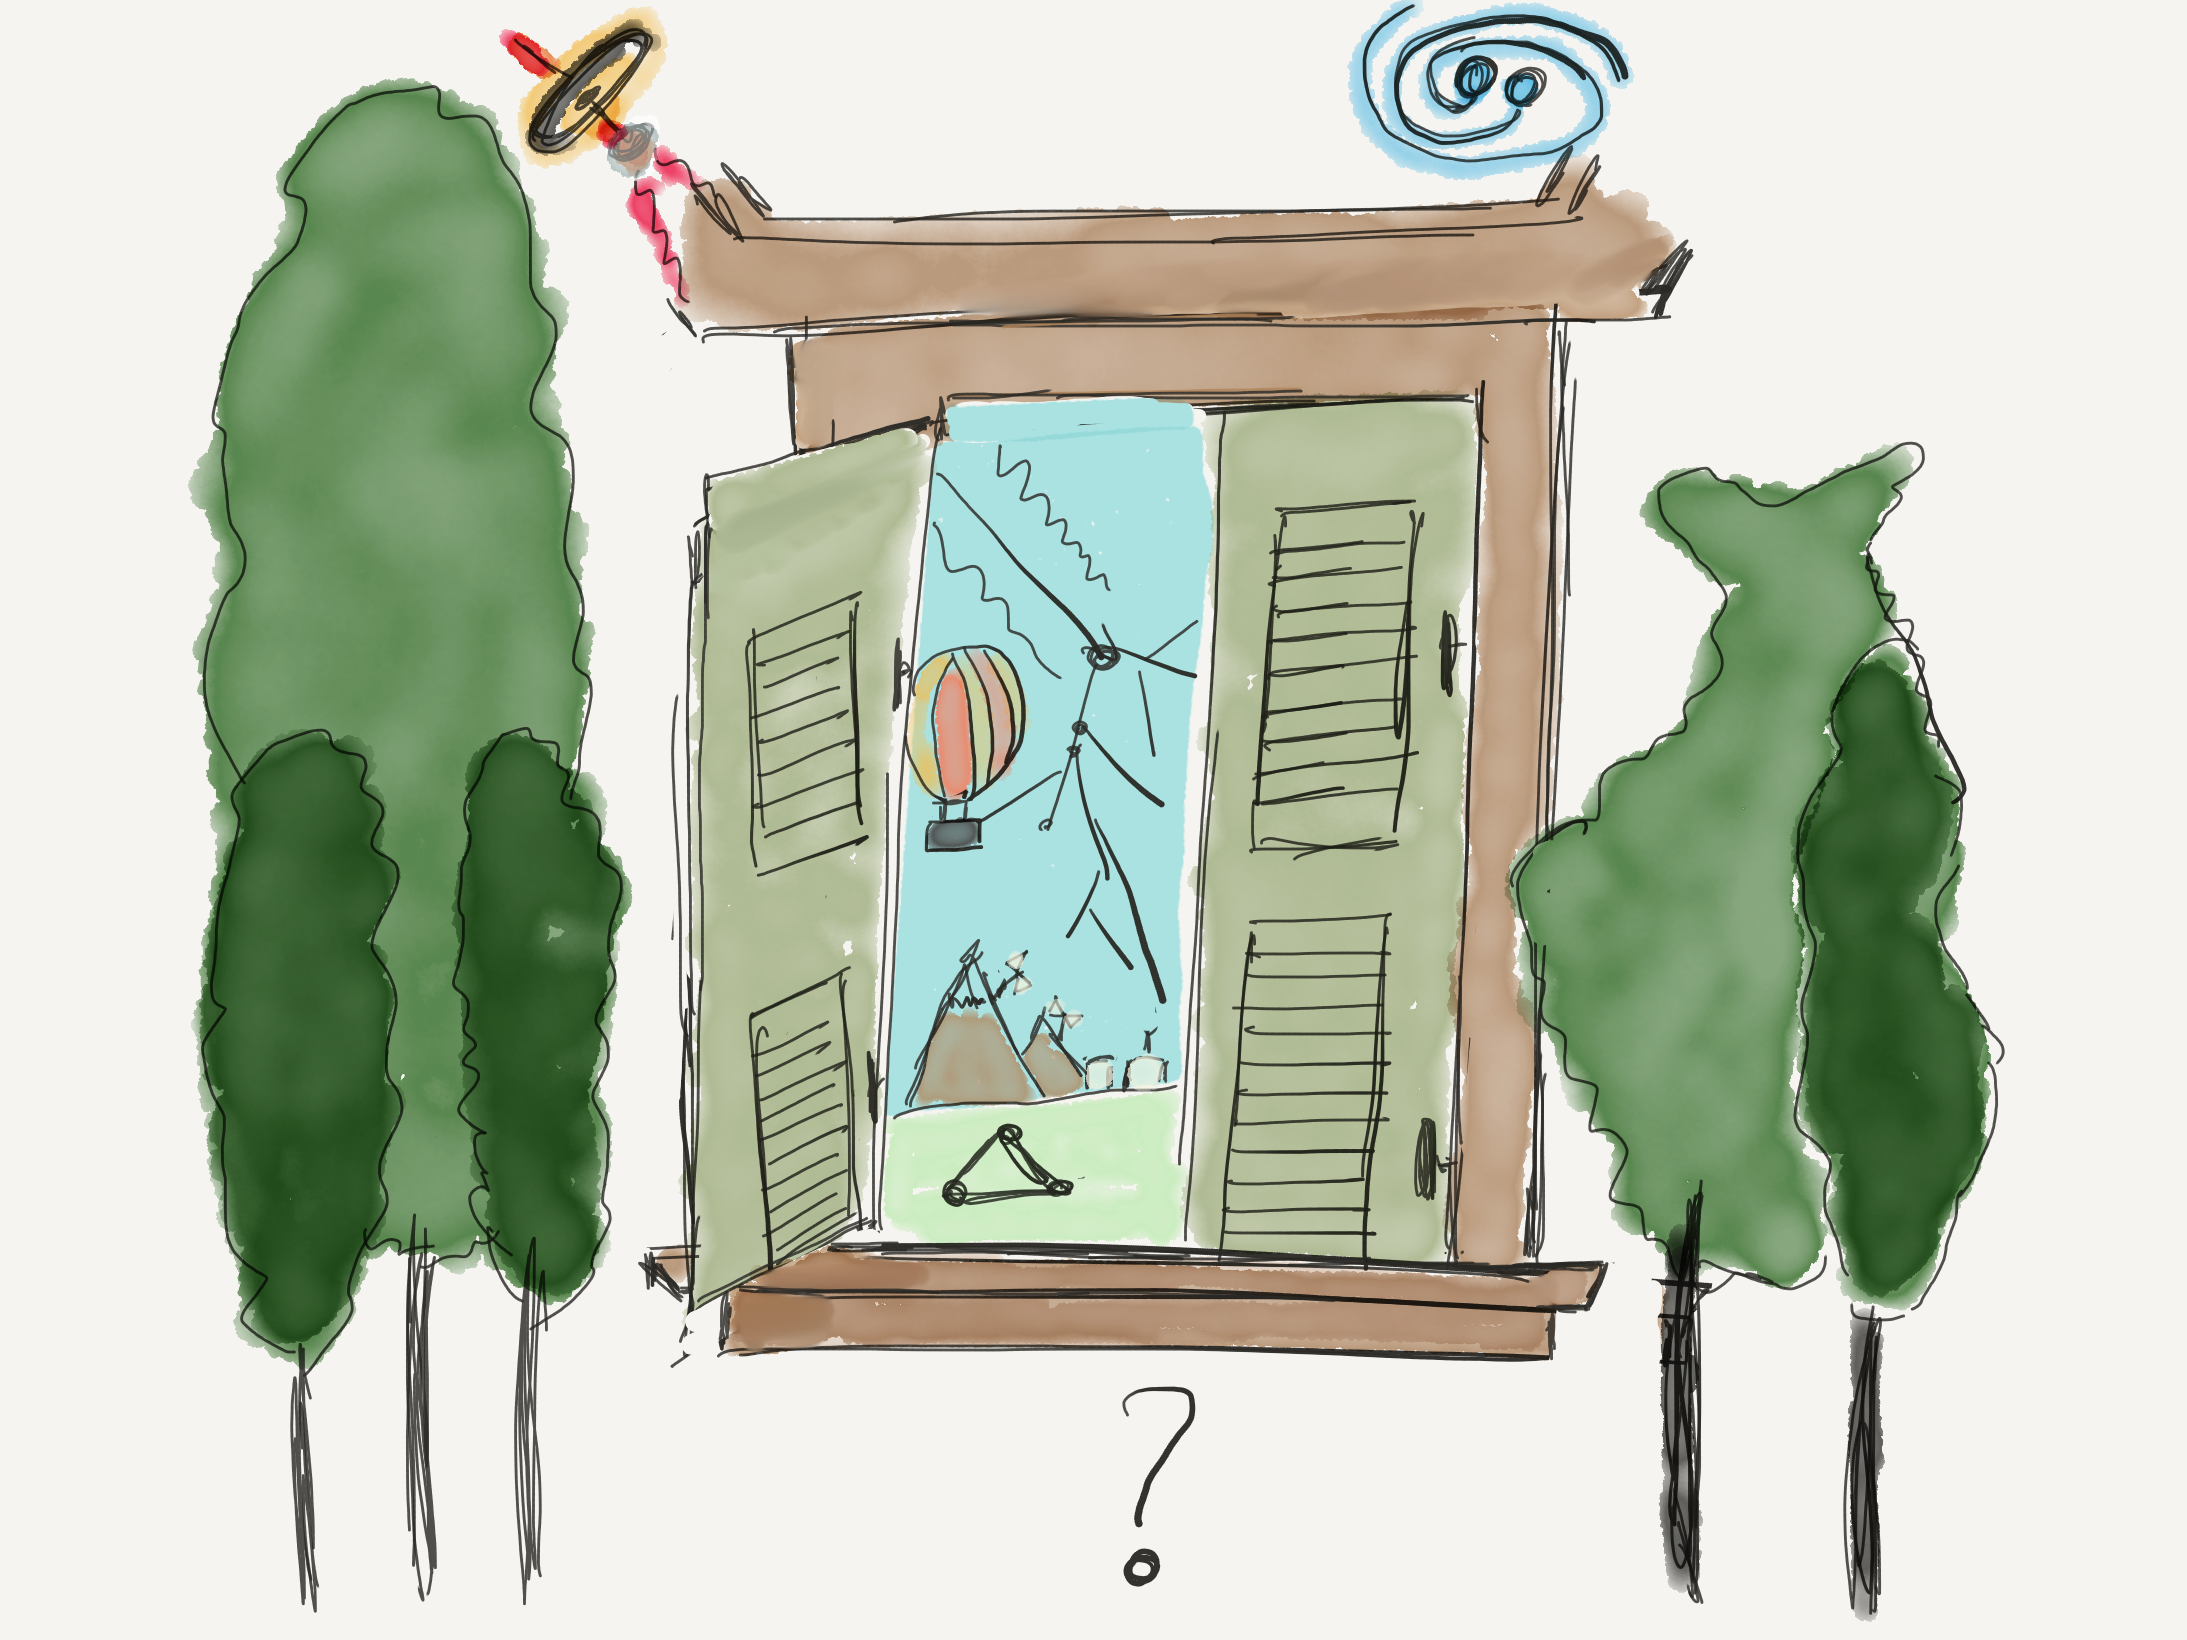
\includegraphics[width=13cm]{thesis_figures/What?.png}
\caption{Window to the inner workings of the Universe is only half opened. (better caption?)}
\label{fig:intro}
\end{figure}
The need to understand how something works or why something is?, is ingrained in every human. While attempting to find answers for these questions one either answers them conclusively or finds oneself asking additional questions stemming from the original. One such question which bothered physicists at the beginning of the 20th century and eventually led to the field of \textit{astro-particle physics} was of so-called "atmosphere electricity" or ionization of air. After the pioneering discoveries by Theodor Wulf~\cite{article_Wulf} and Victor Hess~\cite{Hess:1912srp} who found the increase of this ionization rate with altitude and theorized the origin of this radiation to be not earth but something above our atmosphere, the name \textit{cosmic rays} was coined by Robert Millikan who believed these rays were originating from primary photons. This hypothesis was rejected by the measurements done by Jacob Clay~\cite{Clay:1927I,Clay:1928II} in 1927 who observed a latitude dependence of the intensity of \glspl{CR} concluding this to be a deflection of the primary \glspl{CR} by the geomagnetic field of the earth which indicated that these rays must be charged particles. After this came the efforts of B. Rossi~\cite{rossi1933eigenschaften}, German group~\cite{schmeiser1938harten} and P. Auger~\cite{RevModPhys.11.288} all independently discovering coincident signals in separated Geiger counters which they explained by the counters being struck by an extensive particle shower triggered by a primary \gls{CR}. The phenomenon was named \textit{sciami} by Rossi, \textit{Luftshauer} by the German group and "Auger showers" by Auger and his collaborators. Auger went one step further and estimated the primary energy of the \gls{CR} via his superior setup giving rise to some questions about \glspl{CR} which are yet unanswered, how are they created and where are they coming from. One of the known sources which is the Sun is too close to explain some other high energy \glspl{CR} constantly hitting the Earth's atmosphere. Since then the field has only expanded with numerous experiments set up to characterize these \glspl{CR}. 

The biggest of these experiments which looks for \GLSpl{UHECR} exists in 3000 km$^2$ patch of Argentinian pampa just outside Malargüe called the Pierre Auger Observatory~\cite{Auger:2015}. It uses a combination of 1660 water Cherenkov tanks which form the \gls{SD} of the observatory and observe the air shower particles arriving at the ground along with Fluorescence Telescopes which can look at the development of shower as it travels through the atmosphere. Built primarily to answer the question of the cut-off of the cosmic ray spectrum interpreted as \gls{GZK} limit (or GZK cut-off), the observatory has provided immense contributions not only in the field of \glspl{CR} but also in the fields of Geophysics (elves)~\cite{Mussa_2022}, Dark matter (composition)~\cite{Abreu_2023} and multi-messenger physics (neutrino \& photon searches)~\cite{Aab_2019_point,Auger_photons_2022}. Currently, the \gls{SD} is undergoing an upgrade which will add a scintillator and radio antenna on top of the water Cherenkov tanks further increasing the sensitivity of the observatory especially to the composition of the cosmic rays.

The non-electrical neutrality of the incoming \glspl{CR} provides one of the biggest hindrance for finding their sources. This means that \glspl{CR} do not travel in straight lines from their sources and are affected by the magnetic fields. They can also interact with the matter along the way~\cite{bister2024largescaleanisotropyfluxdemagnification, ALLARD201233}. Combined with the fact that the possible sources are light-years away from us, without knowing the magnetic fields of the Universe it is very hard to detect the sources of \glspl{CR}. \GLSpl{UHEnu} can help in this challenging search for the sources of \glspl{CR}~\cite{UHEcorrelation_2016}. Being electrically neutral and having a very low interaction cross-section these particles can travel large distances unaffected by the intervening matter and magnetic fields. Several scenarios which are discussed later in section~\ref{subsubsec:CRmessengers} describe how the \glspl{UHEnu} can be produced by cosmic-rays and can tell us about their sources. Moreover, \glspl{UHEnu} are also interesting as they can help constrain or explain different production and propagation scenarios for various sources helping us see known astrophysical and cosmogenic objects in a new way. The success of the IceCube Neutrino Observatory, a neutrino detection experiment located at the South Pole, in measuring the first astrophysical neutrinos and the identification of the first steady source NGC 1068~\cite{Icecube_2022} and transient source~\cite{Icecube_txs} have reinvigorated the astro-particle field. The Pierre Auger Observatory has also contributed to the search for \glspl{UHEnu} by trying to detect the \GLSpl{EAS} that can be induced by them. With its stellar sensitivity at high energy, searches at Pierre Auger Observatory have provided some of the strictest upper limits on the diffuse flux of \glspl{UHEnu}~\cite{Aab_2019_diffuse}. This has already led to constrains on various hypothesized models explaining cosmogenic neutrino production.

The last decade with the successes of LIGO/VIRGO~\cite{PhysRevLett.116.061102} in measuring the first gravitational waves and IceCube in detecting the first astrophysical neutrinos has also rekindled a field which displays the true spirit of harmony in science and is called multi-messenger astronomy. The aim of the field is to establish a network that can coalesce all the information available through various messengers via which we can see the Universe and maximise the resources and experiments available at Earth. This also allows us to understand the sources better since the observation or non-observation of different messengers can help constrain the mechanisms behind their functioning. The beginning of this field can be traced back to the observation of the first cosmic rays in conjunction with solar flares, signifying the important role of a cosmic ray observatory like the Pierre Auger Observatory to multi-messenger astronomy. One of the most important success stories of this field is the August 2017 detection of the neutron star collision~\cite{Abbott_2017} first by the LIGO/VIRGO detector since the Gravitational waves are the fastest messengers and then 1.7s later by the Fermi Gamma ray space telescope and INTEGRAL. 11 hours later already alerted by these two experiments the optical counterpart was detected by multiple telescopes like Las Campanas Observatory and the Hubble Space Telescope. The event was also further seen in Ultraviolet (Neil Gehrels Swift Observatory), X-ray (Chandra X-ray Observatory) and radio (Karl G. Jansky Very Large Array). The non observation of neutrinos by both the IceCube and the Pierre Auger Observatory helped reach the important conclusion about the orientation of the jets which is hypothesized to be off-axis i.e. not pointing directly towards the Earth. Since neutrinos and gravitational waves are the fastest of the messengers to reach the Earth, alerts issued by IceCube and LIGO/VIRGO are regularly used to follow up the events with other experiments. Subsequent observations of the blazar TXS 0506+056~\cite{TXS_Multi_2018} with IceCube, FERMI-LAT and MAGIC and the observations of neutrinos from the plane of the Milky Way galaxy~\cite{Galactic_plane_nu_2023} have helped establish the continued importance of multi-messenger astronomy.

In this thesis performance of one of the upgrades of the Pierre Auger Observatory done in 2013 is evaluated in the context of neutrino search. This upgrade consisted of introducing new triggers called \GLS{ToTd} and \GLS{MoPS} to reduce the muonic background and effectively decrease the energy threshold for the array. Such triggers can be particularly important in the context of neutrino searches between zenith angle of $60^\circ$-$75^\circ$ since they help in getting a better signal background separation. The effect of these triggers for both the search of a diffused neutrino flux and point like sources of neutrinos is investigated. The thesis also focuses on maximising the previously done neutrino searches in the zenith region $60^\circ$-$75^\circ$ by investigating and updating the analysis presented in~\cite{Aab_2019_diffuse, gap_note_2013}.

The thesis is structured as follows: The next chapter~\ref{chap:crnNu} gives the theoretical background for \glspl{UHECR} and \glspl{UHEnu} and other important messengers in regard to the Pierre Auger Observatory. It also aims to discuss the various theoretical scenarios involved in their production and propagation. The chapter also aims to summarize the important recent results for these messengers and the various interesting open questions for them. Chapter~\ref{chap:EAS} describes the phenomenon of \glspl{EAS} which is used to indirectly detect both the \glspl{CR} and neutrinos at the Pierre Auger Observatory. To continue with understanding the detection in a more experimental context the following chapter~\ref{chap:setup} gives a detailed description of the Pierre Auger Observatory. The objective of the chapter is to try to give an exhaustive description of all the tools at the Pierre Auger Observatory necessary to detect neutrinos with a particular focus on the \gls{SD} which is of primary concern for the analysis presented in this thesis. A small section is also dedicated to the recently completed AugerPrime upgrade and the exciting potential it offers especially for multi-messenger searches. 

The second part of the thesis is dedicated to the neutrino search in the zenith angular region $ \in 60^\circ$-$75^\circ$, \gls{DGL}. This part begins with chapter~\ref{chap:DGL} that gives a description of the neutrino search in the zenith angular range $60^\circ$-$75^\circ$ which is also the primary focus region for this thesis. The chapter is dedicated to provide a complete description of the choices made for the analysis with the proper reasoning. A \textit{blind} search is performed i.e. the analysis is finalized before the recorded data is used to search for neutrinos. It reports the areas of potential improvements and also communicates the observed improvements to the neutrino identification with the new triggers. The following chapter~\ref{chap:exp_limits_diffuse} discusses the sensitivity of the Pierre Auger Observatory to neutrinos in the investigated zenith angle range. The recorded data is searched to look for neutrinos and due to the non-observance of any neutrino like events, the corresponding upper limits to the diffuse flux of \glspl{UHEnu} are presented with a focus on the observed improvements with the new triggers. The observatory can also detect showers in zenith angle range $\in 75^\circ$-$90^\circ$, \gls{DGH} and up-going showers in the zenith angular region $ \in 90^\circ$-$95^\circ$, \gls{ES} with the \gls{SD} and $\in 90^\circ$-$180^\circ$ with the fluorescence telescopes, but these searches are not performed in this thesis and only their final results are included for comparison and to provide a holistic feel for the neutrino search at Pierre Auger Observatory.

The last part of this thesis presents the sensitivity of the Pierre Auger Observatory to point like sources of \glspl{UHEnu} in chapter~\ref{chap:follow-up}. Due to the non-observance of any neutrinos in the recorded data at the Pierre Auger Observatory an upper limit for point like sources of \glspl{UHEnu} is also shown to be improved with the inclusion of new triggers in the analsis. The limit set by this analysis is also used to calculate an upper limit on the expected neutrino flux for some interesting point source neutrino candidates. All the important results are then finally summarized in chapter~\ref{chap:conc} and a short outlook on the future directions for the analysis and the neutrino search at the Pierre Auger Observatory is put forward. The dissertation is completed by five appendices. The first contains accompanying technical information for neutrino simulations, the second describes the independent work done in this thesis to compare the various hadronic interaction models for neutrino simulations and the third comprises of detailed information about few of the interesting events observed during the analysis. The fourth appendix contains the results of the discrimination analysis performed in this thesis and the fifth contains a technical overview of the changes made to implement the \gls{DGH} neutrino search within the software framework of the Pierre Auger Observatory. 

%%% Local Variables:
%%% mode: latex
%%% TeX-master: "mythesis"
%%% End:
